\documentclass[11pt,a4paper]{article}

\usepackage[utf8]{inputenc}
\usepackage[T1]{fontenc}
\usepackage{lmodern}
\usepackage[margin=2.5cm]{geometry}
\usepackage{amsmath,amssymb}
\usepackage{booktabs}
\usepackage{graphicx}
\usepackage{enumitem}
\usepackage{listings}
\usepackage{xcolor}
\usepackage{float}
\usepackage{pgfplots}
\pgfplotsset{compat=1.16}
\usepackage[hidelinks]{hyperref}

\lstset{
  basicstyle=\ttfamily\scriptsize,
  columns=fixed,
  keepspaces=true,
  breaklines=true,
  frame=single,
  framerule=0.3pt,
  aboveskip=8pt,
  belowskip=8pt
}

\setlist[itemize]{itemsep=2pt, topsep=4pt}
\setlist[enumerate]{itemsep=2pt, topsep=4pt}

\title{Connect 4 AI Agent using Minimax with Alpha-Beta Pruning\\[6pt]
\large Artificial Intelligence -- Assignment 2}
\author{Member 1: Mohamed Ahmed Salama, 23010716\\
Member 2: Omar Assem Ahmed, 23010610\\[8pt]
Alexandria University, Faculty of Engineering\\
Computer and Systems Department}
\date{November 2026}

\begin{document}

\maketitle
\tableofcontents
\newpage

% ------------------------------------------------------------
\section{Introduction}
This report describes a Connect 4 game (human vs.\ computer) implemented in Python.
The board has 7 columns and 6 rows. The game continues until the board is full and the
winner is the player with the greater number of connected-fours. The computer chooses
its moves with minimax with alpha-beta pruning, truncated after $K$ levels (chosen by
the user before the game starts), and a custom heuristic evaluates the states at the
cut-off. The minimax tree of every AI move is printed (console) and shown (GUI),
including the heuristic value of every leaf and, when the option ``show boards'' is
enabled, the board of every leaf.

% ------------------------------------------------------------
\section{Project structure and how to run}
\begin{center}
\begin{tabular}{@{}ll@{}}
\toprule
File & Purpose\\
\midrule
\texttt{board.py} & board representation, moves, windows, counting fours\\
\texttt{minimax.py} & minimax + alpha-beta, tree printing, nodes and time\\
\texttt{heuristic.py} & the heuristic evaluation function\\
\texttt{console.py} & console version of the game\\
\texttt{gui.py} & tkinter GUI with tree panel (bonus)\\
\texttt{benchmark.py} & time/nodes experiments for different $K$\\
\bottomrule
\end{tabular}
\end{center}
Run with \texttt{python3 console.py}, \texttt{python3 gui.py} or \texttt{python3 benchmark.py}.
No external libraries are needed (the GUI needs tkinter).

% ------------------------------------------------------------
\section{Data structures}
\begin{itemize}
  \item \textbf{Board:} a list of lists with 6 rows and 7 columns. 0 = empty, 1 = human
  (X, red), 2 = AI (O, yellow). Row 0 is the top row. \texttt{drop\_piece} returns a
  \emph{copy} of the board with the disc added, so parent states are never modified
  while the search goes deeper.
  \item \textbf{Windows:} \texttt{get\_windows} returns a list of the 69 groups of four
  consecutive cells (horizontal, vertical and both diagonals). Both the score and the
  heuristic are computed from these windows.
  \item \textbf{Column order:} the list \texttt{ORDER = [3, 2, 4, 1, 5, 0, 6]} (centre
  first). Centre columns are usually better, so trying them first produces more
  cut-offs.
  \item \textbf{Tree:} a list of strings, one per node, indented by depth.
  \texttt{choose\_move} returns a dictionary with \texttt{col}, \texttt{value},
  \texttt{nodes}, \texttt{time} and \texttt{tree}.
  \item \textbf{Statistics:} a dictionary holding the node counter, shared by the
  recursive calls.
\end{itemize}

% ------------------------------------------------------------
\section{Algorithm}
\subsection{Minimax with alpha-beta pruning}
The AI is the MAX player and the human is the MIN player. The recursive function
\texttt{minimax(board, depth, alpha, beta, maximizing, \dots)} works as follows:
\begin{enumerate}
  \item If the board is full, return the real result
  $(\text{AI fours}-\text{human fours})\times 1000$ (a full node). The factor 1000 makes
  real outcomes always more important than heuristic estimates.
  \item Otherwise, if \texttt{depth == 0}, return the heuristic value
  \texttt{evaluate(board)} (a leaf).
  \item Otherwise try every valid column (centre first). MAX takes the largest child
  value and raises $\alpha$; MIN takes the smallest child value and lowers $\beta$.
  \item When $\alpha \ge \beta$ the remaining columns cannot change the decision, so they
  are skipped (pruned) and printed in the tree.
\end{enumerate}
The initial call is \texttt{minimax(board, K, -inf, +inf, True)}, and the column with the
best value at the root is played. Plain minimax is the same function with pruning
switched off (parameter \texttt{prune=False}); it is used only for the comparison in
Section~\ref{sec:analysis}.

\subsection{Complexity}
With branching factor $b \le 7$, plain minimax visits about $b^{K}$ nodes. Alpha-beta
visits about $b^{K/2}$ in the best case, which needs good move ordering. This is why the
centre-first order is used.

\subsection{Depth cut-off}
The full game tree has about $10^{35}$ nodes, so the search stops after $K$ levels and
evaluates the states with the heuristic. $K$ is read from the user before the game
starts (console prompt / GUI spin box).

% ------------------------------------------------------------
\section{Heuristic function}
The heuristic returns a larger number when the AI is closer to winning and a smaller
(more negative) number when the human is closer to winning. It is computed in a single
pass over the 69 windows. A window that contains discs of only one player is still a
possible future four for that player; a window with discs of both players can never
become a four and is ignored. This is also the idea of ``candidate points'': empty
cells that can still complete a four.

\begin{center}
\begin{tabular}{@{}lcc@{}}
\toprule
Feature (per window) & AI & Human\\
\midrule
Completed four (current score) & $+100$ & $-100$\\
Open three: 3 own discs + 1 empty & $+10$ & $-12$\\
Open two: 2 own discs + 2 empty & $+3$ & $-4$\\
Each disc in the centre column & $+4$ & $-4$\\
\bottomrule
\end{tabular}
\end{center}

\paragraph{Why these weights.}
\begin{itemize}
  \item A completed four is the real objective of the game (the winner has more fours),
  so it has the largest weight. The three-disc and two-disc windows are only steps toward
  it, so they get ten times and thirty times less.
  \item The human's open threes and twos weigh slightly more than the AI's (12 vs.\ 10,
  4 vs.\ 3). This makes the AI a little defensive: it prefers blocking a human threat to
  building an equal one of its own.
  \item The centre column belongs to the largest number of windows, so a disc there is
  worth more than a disc on the edge.
  \item The maximum heuristic value stays much smaller than 1000, so a real result at a
  full board always dominates.
  \item The heuristic is fast: one loop over 69 small windows plus six centre cells. This
  matters because it runs on every leaf.
\end{itemize}

\paragraph{Worked example.} Consider the leaf below (the human has just played column 4):
\begin{lstlisting}
. . . . . . .
. . . . . . .
. . . . . . .
. . . O . . .
. . . O . . .
. . X X X . .
\end{lstlisting}
Human windows in the bottom row: columns 1--4 and 2--5 each contain three X and one empty
($2\times(-12)=-24$); columns 0--3 and 3--6 each contain two X and two empty
($2\times(-4)=-8$). AI windows: the vertical window in column 3 over rows 1--4 contains two
O and two empty ($+3$). Centre column: X $-4$, O $+4$, O $+4$ $=+4$. Total:
$-24-8+3+4=-25$, exactly the value printed in the tree of Section~\ref{sec:samples}.

% ------------------------------------------------------------
\section{Sample runs and minimax trees}\label{sec:samples}
\subsection{Tree format}
Every line is one node, indented by its depth:
\begin{itemize}
  \item \texttt{col c MAX/MIN value=v alpha=a beta=b}: an internal node reached by playing
  column $c$; $v$ is its minimax value and $a$, $b$ the alpha and beta bounds when the
  node finished.
  \item \texttt{col c LEAF h=v}: a leaf at depth $K$ with its heuristic value (and
  optionally the board the heuristic evaluated, printed below the line).
  \item \texttt{col c FULL h=v}: a terminal node (full board) with the real score
  $\times 1000$.
  \item \texttt{pruned cols [...]}: the columns that alpha-beta did not explore.
\end{itemize}

\subsection{Sample 1: $K=2$ with boards}
Position before the AI move (human played column 3, AI column 3, human column 2; the AI
(O) is to move):
\begin{lstlisting}
. . . . . . .
. . . . . . .
. . . . . . .
. . . . . . .
. . . O . . .
. . X X . . .
0 1 2 3 4 5 6
\end{lstlisting}
Beginning of the tree (the first child of the root, with the board and heuristic value of
its first five leaves):
\begin{lstlisting}
root MAX value=-9 alpha=-9 beta=inf
    col 3 MIN value=-25 alpha=-inf beta=-25
        col 3 LEAF h=-12
            . . . . . . .
            . . . . . . .
            . . . X . . .
            . . . O . . .
            . . . O . . .
            . . X X . . .
            0 1 2 3 4 5 6
        col 2 LEAF h=-13
            . . . . . . .
            . . . . . . .
            . . . . . . .
            . . . O . . .
            . . X O . . .
            . . X X . . .
            0 1 2 3 4 5 6
        col 4 LEAF h=-25
            . . . . . . .
            . . . . . . .
            . . . . . . .
            . . . O . . .
            . . . O . . .
            . . X X X . .
            0 1 2 3 4 5 6
        col 1 LEAF h=-21
            . . . . . . .
            . . . . . . .
            . . . . . . .
            . . . O . . .
            . . . O . . .
            . X X X . . .
            0 1 2 3 4 5 6
        col 5 LEAF h=-17
            . . . . . . .
            . . . . . . .
            . . . . . . .
            . . . O . . .
            . . . O . . .
            . . X X . X .
            0 1 2 3 4 5 6
\end{lstlisting}
The AI finally chooses column 4 (value $-9$), which blocks the human's bottom row; the
whole search expanded 34 nodes.

\subsection{Sample 2: the same position, $K=2$, whole tree without boards}
This shows the pruning (the root's children for columns 1, 5, 0 and 6 are cut after only
one or two leaves, because their first reply already gives the human a value worse than
the $-9$ the AI can guarantee):
\begin{lstlisting}
root MAX value=-9 alpha=-9 beta=inf
    col 3 MIN value=-25 alpha=-inf beta=-25
        col 3 LEAF h=-12
        col 2 LEAF h=-13
        col 4 LEAF h=-25
        col 1 LEAF h=-21
        col 5 LEAF h=-17
        col 0 LEAF h=-13
        col 6 LEAF h=-9
    col 2 MIN value=-23 alpha=-25 beta=-23
        col 3 LEAF h=-7
        col 2 LEAF h=-3
        col 4 LEAF h=-23
        col 1 LEAF h=-19
        col 5 LEAF h=-15
        col 0 LEAF h=-11
        col 6 LEAF h=-7
    col 4 MIN value=-9 alpha=-23 beta=-9
        col 3 LEAF h=-5
        col 2 LEAF h=-9
        col 4 LEAF h=-5
        col 1 LEAF h=-9
        col 5 LEAF h=-1
        col 0 LEAF h=-9
        col 6 LEAF h=-1
    col 1 MIN value=-12 alpha=-9 beta=-12
        col 3 LEAF h=-8
        col 2 LEAF h=-12
        pruned cols [4, 1, 5, 0, 6]
    col 5 MIN value=-12 alpha=-9 beta=-12
        col 3 LEAF h=-12
        pruned cols [2, 4, 1, 5, 0, 6]
    col 0 MIN value=-12 alpha=-9 beta=-12
        col 3 LEAF h=-12
        pruned cols [2, 4, 1, 5, 0, 6]
    col 6 MIN value=-16 alpha=-9 beta=-16
        col 3 LEAF h=-16
        pruned cols [2, 4, 1, 5, 0, 6]
\end{lstlisting}

\subsection{Sample 3: a complete game}\label{sec:game}
This sample is a complete game played with the GUI (\texttt{python3 gui.py}) at $K=4$.
The human (red) played first and the AI (yellow) second, and the game continued until the
board was full, i.e.\ 21 moves for each player. The option ``show boards in tree'' was
switched off in this run to keep the 21 trees short (trees with boards are shown in
Sample~1). The complete trees of all 21 AI moves were written to \texttt{tree\_log.txt}
by the GUI during this game. The final position is shown in Figure~\ref{fig:final}: the
final score is \textbf{You 1 -- AI 5}, so the AI wins.

\begin{figure}[H]
\centering
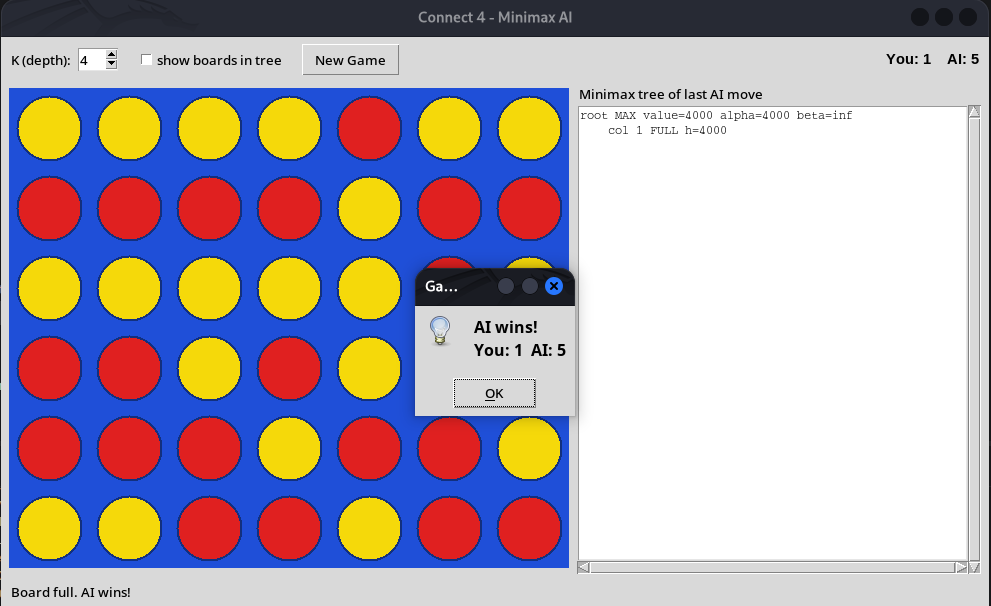
\includegraphics[width=0.95\textwidth]{final_game.png}
\caption{Screenshot of the GUI at the end of the game ($K=4$): the board is full, the
tree panel shows the tree of the last AI move, and the final score is You 1 -- AI 5.}
\label{fig:final}
\end{figure}

Table~\ref{tab:game} lists, for every AI move, the column that was played and the minimax
value of the root (the value is taken from the first line of each printed tree).

\begin{table}[H]
\centering
\small
\begin{tabular}{@{}ccrccrccr@{}}
\toprule
Move & Col & Value & Move & Col & Value & Move & Col & Value\\
\midrule
1  & 3 & $-12$ & 8  & 2 & $-2$  & 15 & 6 & $19$\\
2  & 3 & $-17$ & 9  & 0 & $1$   & 16 & 6 & $31$\\
3  & 3 & $-17$ & 10 & 4 & $0$   & 17 & 5 & $121$\\
4  & 1 & $-20$ & 11 & 5 & $5$   & 18 & 0 & $124$\\
5  & 2 & $-21$ & 12 & 4 & $23$  & 19 & 0 & $310$\\
6  & 2 & $-7$  & 13 & 4 & $19$  & 20 & 1 & $4000$\\
7  & 4 & $-5$  & 14 & 6 & $19$  & 21 & 1 & $4000$\\
\bottomrule
\end{tabular}
\caption{Column chosen and root minimax value for each of the 21 AI moves ($K=4$).}
\label{tab:game}
\end{table}

What the trees of this game show:
\begin{itemize}
  \item The root value is negative at the beginning (the human moves first and takes the
  centre) and becomes positive from move 9, when the AI has built more open windows than
  the human.
  \item In move 4 the first candidate, column 2, has the value $-102$. Its leaves have
  values around $-100$ or lower, i.e.\ they contain a completed human four (weight
  $-100$). The AI therefore avoids column 2 and plays column 1 (value $-20$).
  \item From move 17 the root values are above 100: the leaves already contain completed
  AI fours (weight $+100$ each).
  \item In the last tree the value $4000$ equals $(5-1)\times 1000$, which is exactly the
  final score of Figure~\ref{fig:final}.
  \item Pruning is visible in every tree through the \texttt{pruned cols} lines.
\end{itemize}

The trees of the last three AI moves are short enough to be printed completely. In move 19
only columns 0 and 1 still have free cells, so the tree is very small:
\begin{lstlisting}
===== AI move 19 (K=4) =====
root MAX value=310 alpha=310 beta=inf
    col 1 MIN value=100 alpha=-inf beta=100
        col 1 MAX value=100 alpha=100 beta=inf
            col 1 MIN value=100 alpha=-inf beta=100
                col 1 LEAF h=100
                col 0 LEAF h=100
            col 0 MIN value=10 alpha=100 beta=10
                col 1 LEAF h=10
        col 0 MAX value=300 alpha=300 beta=100
            col 1 MIN value=300 alpha=-inf beta=100
                col 1 LEAF h=300
    col 0 MIN value=310 alpha=100 beta=310
        col 1 MAX value=310 alpha=310 beta=inf
            col 1 MIN value=310 alpha=100 beta=310
                col 1 LEAF h=310

===== AI move 20 (K=4) =====
root MAX value=4000 alpha=4000 beta=inf
    col 1 MIN value=4000 alpha=-inf beta=4000
        col 1 MAX value=4000 alpha=4000 beta=inf
            col 1 FULL h=4000

===== AI move 21 (K=4) =====
root MAX value=4000 alpha=4000 beta=inf
    col 1 FULL h=4000
\end{lstlisting}

% ------------------------------------------------------------
\section{Time and nodes analysis}\label{sec:analysis}
\texttt{benchmark.py} plays one complete game for each $K$ (the human is a random player,
fixed seed) with alpha-beta pruning and with plain minimax. Plain minimax at $K=5$ was
skipped because it takes too long.

\begin{table}[H]
\centering
\begin{tabular}{@{}clrrrr@{}}
\toprule
$K$ & Algorithm & Total nodes & Nodes/move & Time (s) & Time/move (s)\\
\midrule
1 & alpha-beta & 125   & 6.0    & 0.005 & 0.0002\\
1 & plain      & 125   & 6.0    & 0.004 & 0.0002\\
2 & alpha-beta & 417   & 19.9   & 0.010 & 0.0005\\
2 & plain      & 742   & 35.3   & 0.020 & 0.0010\\
3 & alpha-beta & 1505  & 71.7   & 0.037 & 0.0018\\
3 & plain      & 4102  & 195.3  & 0.111 & 0.0053\\
4 & alpha-beta & 6162  & 293.4  & 0.143 & 0.0068\\
4 & plain      & 28829 & 1372.8 & 0.773 & 0.0368\\
5 & alpha-beta & 14940 & 711.4  & 0.337 & 0.0160\\
\bottomrule
\end{tabular}
\caption{Nodes and time for one game against a random human (21 AI moves).}
\label{tab:bench}
\end{table}

\begin{figure}[H]
\centering
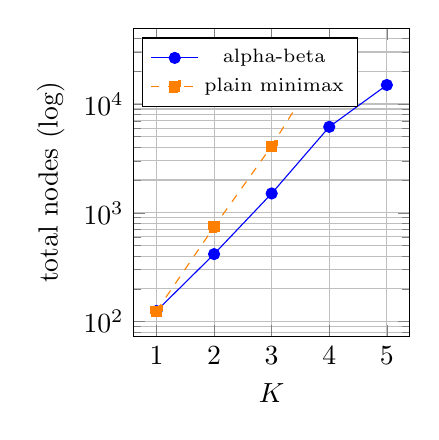
\begin{tikzpicture}
\begin{axis}[width=0.42\textwidth, height=5.5cm, ymode=log, grid=both,
  xlabel={$K$}, ylabel={total nodes (log)}, xtick={1,2,3,4,5},
  legend pos=north west, legend style={font=\scriptsize}]
\addplot[blue, mark=*] coordinates {(1,125) (2,417) (3,1505) (4,6162) (5,14940)};
\addplot[orange, dashed, mark=square*] coordinates {(1,125) (2,742) (3,4102) (4,28829)};
\legend{alpha-beta, plain minimax}
\end{axis}
\end{tikzpicture}
\hfill
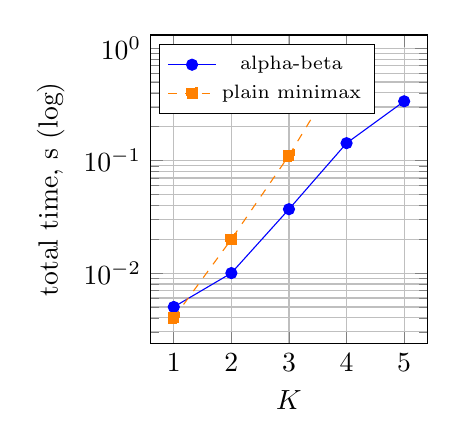
\begin{tikzpicture}
\begin{axis}[width=0.42\textwidth, height=5.5cm, ymode=log, grid=both,
  xlabel={$K$}, ylabel={total time, s (log)}, xtick={1,2,3,4,5},
  legend pos=north west, legend style={font=\scriptsize}]
\addplot[blue, mark=*] coordinates {(1,0.005) (2,0.010) (3,0.037) (4,0.143) (5,0.337)};
\addplot[orange, dashed, mark=square*] coordinates {(1,0.004) (2,0.020) (3,0.111) (4,0.773)};
\legend{alpha-beta, plain minimax}
\end{axis}
\end{tikzpicture}
\caption{Total nodes and total time against $K$ (log scale).}
\label{fig:bench}
\end{figure}

\paragraph{Discussion.}
\begin{itemize}
  \item At $K=1$ both algorithms expand the same nodes, because a cut-off needs at least
  two levels.
  \item Pruning removes more work as $K$ grows: plain minimax expands $1.8\times$ ($K=2$),
  $2.7\times$ ($K=3$) and $4.7\times$ ($K=4$) more nodes than alpha-beta, and takes about
  $2\times$, $3\times$ and $5.4\times$ more time.
  \item Both curves are exponential, but alpha-beta grows more slowly (about
  $2.4$--$4\times$ per extra level, plain about $5.5$--$7\times$), so with alpha-beta a
  deeper $K$ is affordable: at $K=5$ the AI needs only about 0.016\,s per move.
  \item Time follows nodes almost linearly, because every node costs a board copy and
  every leaf a heuristic evaluation.
  \item The numbers come from one game per row, so they show the trend rather than exact
  values. The node counts are deterministic; the times depend on the machine. Tree
  printing was switched off for the benchmark (it adds string work to every node).
\end{itemize}

% ------------------------------------------------------------
\section{Quality of the heuristic}
To check that the heuristic plays reasonably, the AI (with the final heuristic and with
the placeholder ``score difference only'' heuristic) played 20 games against a random
human for each $K$. In all 100 games with both heuristics the AI won.

\begin{table}[H]
\centering
\begin{tabular}{@{}crrrr@{}}
\toprule
 & \multicolumn{2}{c}{Final heuristic} & \multicolumn{2}{c}{Score-difference only}\\
\cmidrule(lr){2-3}\cmidrule(lr){4-5}
$K$ & AI fours & human fours & AI fours & human fours\\
\midrule
1 & 10.9 & 0.95 & 10.6 & 3.75\\
2 & 8.6  & 0.55 & 10.1 & 0.85\\
3 & 9.3  & 0.85 & 11.1 & 1.8\\
4 & 9.4  & 0.45 & 10.1 & 0.85\\
5 & 9.9  & 0.55 & 10.9 & 1.0\\
\bottomrule
\end{tabular}
\caption{Average number of connected-fours per game, 20 games per row.}
\label{tab:heur}
\end{table}

The final heuristic lets the human make fewer fours than the placeholder in every row (it
is more defensive), and at $K=1$ it is clearly better. For $K\ge 2$ it gives up a few of
the AI's own fours against a random opponent. In a head-to-head test of the two
heuristics (both at the same $K$, random opening, both colours), the results were about
equal: the average margin was 0.0 fours per game at $K=3$ and $+0.65$ for the final
heuristic at $K=4$ (20 games each). We therefore claim a reasonable and defensive
heuristic, not a large improvement over the simple one; tuning the weights with more
games would be the next step.

% ------------------------------------------------------------
\section{Assumptions}
\begin{itemize}
  \item The board is 7 columns $\times$ 6 rows; the human plays first (red/X), the AI
  second (yellow/O).
  \item The game ends only when the board is full (no early stop at the first four).
  \item A line of five or more discs counts as several fours, because every window of four
  cells is counted (e.g.\ five in a row = 2 fours).
  \item At a full board the value is $(\text{AI fours}-\text{human fours})\times 1000$;
  equal numbers of fours is a draw.
  \item The human is asked for a column number 0--6; invalid or full columns are rejected
  and asked again.
\end{itemize}

% ------------------------------------------------------------
\section{Extra work}
\begin{itemize}
  \item A tkinter GUI: click on a column to play, live score, spin box for $K$,
  nodes/time/value of every AI move.
  \item The minimax tree is shown in a panel of the GUI (with an option to show the
  boards), printed to the console and saved to \texttt{tree\_log.txt}.
  \item A benchmark script comparing alpha-beta with plain minimax for several $K$ and
  writing \texttt{benchmark\_results.csv}.
  \item Centre-first move ordering to increase pruning.
\end{itemize}

% ------------------------------------------------------------
\section{Conclusion}
The agent plays complete games with minimax and alpha-beta pruning, prints a traceable
tree with heuristic values and boards, and takes $K$ as a parameter. In the complete game
of Section~\ref{sec:game} it beat the human 5 to 1 at $K=4$. Alpha-beta pruning reduced
the nodes by up to $4.7\times$ at $K=4$ compared with plain minimax, making depths of 5
and more practical in plain Python.

\end{document}